%\chapter{Fonctionnement général}
%\section{Explication et justification de l'infrastructure}
%\subsection{Général}
%Nous disposons de deux machines pour mettre en place l'infrastructure.
%Cela limite les choix d'architectures possible. Nous nous sommes tourné vers une 
%architecture avec un serveur de centralisation des logs/flux, et un serveur 
%d'indexation et d'exploitation de ces \gls{logs}. C'est une configuration assez standard
%lorsque l'on met en place une pile ELK.
%
%Cette configuration présente l'avantage de répartir la charge de travail de manière 
%assez satisfaisante.Les deux points \textit{chauds} étant la réception des logs 
%(~20-30 millions de lignes par jours) et le traitement de ces logs \textit{nettoyés}.
%
%
%\begin{figure}[H]
%\center
%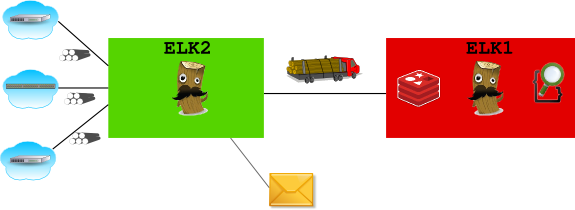
\includegraphics[width=1\textwidth]{stacksimple.png}
%\label{fig:elkstack1}
%\caption{Notre pile ELK}
%\end{figure}
%
%Il est encore possible en cas de besoin de répartir un peu mieux la charge
%en déportant Kibana sur ELK2. Cependant son empreinte mémoire n'est pas très élevée
%et ses besoins en processeur assez ponctuels, ce n'est donc pas un vrai problème.\\[5mm]
%
%Il est possible de faire fonctionner logstash en temps qu'agent, soit en l'installant
%directement sur un matériel, soit en le compilant spécifiquement pour un materiel.
%
%Cela n'a pas été nécessaire puisque l'infrastructure réseau de Lorraine disposait 
%déjà un système complètement fonctionnel sur syslog-ng\footnote{un système d'agent 
%assez avancé permettant la centralisation de log}. 
%Depuis très récemment (encore en beta à l'écriture de ces lignes) syslog-ng est 
%capable d'envoyer ses \gls{logs} vers Elasticsearch, cependant la version de syslog-ng
%installée sur les équipements ne permet actuellement pas de le faire.
%
%Sans entrer dans les détails, cette solutions n'aurait de toute façon pas été retenu,
%car elle impliquait de centraliser et traiter les logs sur la même machine. Ce qui
%aurait probablement eu des effets dramatiques sur les performances, ne parlons pas 
%de la résilience.
%
%Des informations concernant les infrastructures ont été distillées au long des différents
%chapitres, vous trouverez en annexe la \hyperref[]{configuration de logstash elk2},
%la configuration pour \hyperref[]{Logstash elk1}, le mapping des index \hyperref[]{d'état} et 
%de \hyperref[]{firewall}. 
%
%\subsubsection{Redis}
%Nous nous servons de Redis comme d'un tampon (buffer), Logstash d'ELK2 envoie ses 
%données vers Redis situé sur ELK1. Ces données sont ensuite récupérées sur par Logstash
%d'ELK1 qui les envoie sur Elasticsearch.
%
%L'intérêt d'avoir un Redis entre le Logstash ELK2 et Elasticsearch
%est de lisser le trafic. Si Elasticsearch ne peut pas traiter immédiatement 
%les données qui lui sont envoyées \footnote{lors d'une latence disque dur ou de l'utilisation
%intensive du processeur, etc} la file d'attente de Logstash serait immédiatement 
%encombrée. Pour prévenir la perte de donné on ajoute un tampon au milieu qui sauvegardera
%temporairement les données, le temps que Elasticsearch soit à nouveau joignable.\footnote{en 
%cas d'extinction d'Elasticsearch, Redis saturera la RAM puis la swap du serveur en
%quelques heures, au mieux. Il faut donc intervenir vite.}
%
%Sa configuration (\textbf{très simple}) est disponible en annexes.
\chapter{Synthèse}
\section{Analyse des performances}
Globalement en fin de stage, l'infrastructure ELK fonctionne comme demandé.
Mais, la marge de manœuvre sur l'infrastructure, n'est pas très importante.

ELK2 fonctionne très bien, nous pourrions même ajouter plus de trafic et/ou faire
un tri plus drastique (consommateur en CPU) sur les logs. 
La ressource la plus exploité est le réseau mais la aussi il y a une \textbf{très} grande marge.
\footnote{carte réseau Gigabit}
Voir les graphiques \gls{Munin} associés :  p\pageref{fig:elk2cpu} \\[3mm]


Ça va un peu moins bien du coté ELK1. Elasticsearch est un logiciel, gourmand, particulièrement
pour de gros volumes de données. 

Les 12Go de RAM ne sont pas de trop. 8 sont en permanence utilisés avec des variations
importantes, notamment en fonction de l'utilisation de Redis. Voir p\pageref{fig:elk1memory}

Le disque dur malgré, ses 15000tr/min est également un goulot d'étranglement. Lors
d'une grosse recherche avec Kibana, les temps d'accès sont souvent la cause de ralentissements.
Ces effets étant très ponctuels Munin ne les détecte pas.

On pourrait penser en voyant le graphique processeur p\pageref{fig:elk1cpu}, que 
l'on dispose d'une très large marge, mais il s'agit d'un effet d'optique. 
Là aussi Munin n'est pas assez précis pour capter les variations ponctuelles, 
lors d'une recherche, il est fréquent que les 12 cœurs soient entièrement utilisés.
On voit un tout petit peu l'utilisation augmenter vers la fin, lors d'un stress test.\\[3mm]

Attention, l'infrastructure n'est pas pour autant au bord du grouffre, elle est juste
bien dimensionnée pour pouvoir fonctionner avec quelques utilisateurs concurrents et
quelques dizaines de millions de \gls{logs} envoyés par jours, comme c'est le cas actuellement.


\section{Améliorations}
\subsection{Sécurité et déploiement}
Je n'ai pas particulièrement mis en place de dispositifs pour sécuriser 
l'accès à l'infrastructure. Les machines sont à jour et isolés sur un VLAN. 

Mais il est possible de faire mieux au niveau des applications comme par exemple 
ajouter un proxy SSL devant Kibana.

Il est possible de communiquer de syslog-ng vers Logstash par SSL.

Enfin concernant la sécurisation de Redis un bon début est de commencer par écouter 
une seule IP et non pas  0.0.0.0 (toutes).

Concernant Elasticsearch il n'y a pas d'alternative\footnote{la société semble avoir récemment développer
le produit payant : Shield, qui apporterait une couche de sécurtité} il faut l'isoler au maximum du 
reste du réseau.

L'installation n'a pas été automatisée, il faudra le faire, avec Saltstak, logiciel
utilisé par l'équipe Lothaire.
\subsection{Tuning Elasticsearch}
Les possibilités d'optimisations avec Elasticsearch sont nombreuses et toutes n'ont pas été
étudiées. Voici une liste non exhaustive des pistes envisageables : Limiter le nombre de shards (ce qui pourrait
augmenter les performances, notamment les accès), diminuer le nombre de champs et/ou 
d'informations enregistrées afin de diminuer la taille de nos index.

On peut sans doute améliorer le mapping actuel pour mieux le faire correspondre aux
besoins de l'équipe Lothaire (analyseurs particuliers, ajouter des champs non analysés,etc)


%\subsection{Meilleure structuration du rapport}
%L'erreur majeure de ce rapport est d'avoir voulu lié rapport et tutoriel pour l'équipe.
%Un mauvais choix qui s'avère un peu catastrophique pour la lisibilité de l'ensemble
%et qui me force à très sérieusement retravailler ce rendu, à la dernière minute\ldots
%
